%\documentclass[12pt]{report}
%\usepackage{kjfsty}
%\begin{document}
%\onehalfspacing
%
%\tableofcontents
%\cleardoublepage

\setcounter{chapter}{4}
\chapter[Short Injector Quantum Cascade Lasers]{Short Injector \\ Quantum Cascade Lasers}

For QC lasers, the ultimate measure of performance is wall-plug efficiency: quite simply, power out for power in.  And up to only a few years ago, even the best lasers reported in the literature had abysmal wall-plug efficiencies---at most, in the range of a few percent.  Improvement in wall-plug efficiencies will make more applications more accessible; across the board, regardless of the application specifics, more efficient lasers will enhance QC technology's utility.  For example, more efficient lasers ultimately mean lasers that are capable of higher output power.  High power lasers are certainly of paramount interest for infrared-based defense countermeasures, but high power is also needed for such things as lidar, which has a diverse array of applications.  For applications where Watt-level output power is not needed---several methods of trace gas sensing, for example---low input power is often a requirement.

Certainly, the QC field has devoted considerable effort to improving laser performance; along with our understanding of the physical mechanisms at work in QC lasers, performance has improved substantially.  Of chief concern in the initial QC work was achieving population inversion; to realize the first QC laser \cite{Faist:Science:1994}, Faist \emph{et al.} sought to maximize population inversion by using spatially-delocalized upper and lower energy states for the laser transition.  Dubbed a ``diagonal transition'' design, the consequence of such spatial separation---reduced oscillator strength \cite{Faist:Nature:1997:oscillator}---was soon realized.  As a result, ``vertical transitions,'' those where the energy states share the same physical space, were investigated \cite{Faist:APL:1995:vertical}, and performance improvements were realized \cite{Sirtori:APL:1996:vertical}.  Later, the importance of resonant tunneling through the injector barrier was identified \cite{Sirtori:JQE:1998}, and the active region was modified to include a narrow, first active region well to enhance coupling \cite{Faist:APL:1996:coupling}.  The result was a ``hybrid'' active region design that had the appearance of a somewhat diagonal yet somewhat vertical optical transition.  Further performance improvements were again realized \cite{Gmachl:APL:1998:magic} from this insight.

The so-called ``double-phonon'' structure, a 2001 design advance \cite{Hofstetter:APL:2001:2phonon}, led to the first CW room temperature QC laser \cite{Beck:Science:2002}.  Here, a structural modification is again made to the QC active region.  The double-phonon active region is composed of at least three wide quantum wells, where each of the three active region quantum ground states are spaced sequentially one longitudinal optical (LO) phonon energy apart; this allows enhanced relaxation out of the lower laser state \cite{Beck:Science:2002}.  The extra energy drop imparted by the secondary LO phonon transition also mitigates lower laser level thermal backfilling \cite{Howard:JQE:2008}.

More recent performance advances have primarily been demonstrated through improved understanding and implementation of thermal management strategies; QC stacks in a buried heterostructure waveguide mounted epitaxial-side down on diamond submounts have surpassed watt-level power in continuous wave mode at room temperature \cite{Lyakh:CLEO:2008}.  While impressive, these lasers are implemented with designs that are simply derivatives of the double-phonon QC strategy.  Since 2001, no significant performance improvement has been realized by implementing a fundamentally superior QC design.

While much attention has been paid to improving QC performance by modifications to the \emph{active region} structure, in this chapter, I focus on a re-examination of the role of \emph{injector regions} in QC laser performance.  Injectors play numerous roles important to QC laser operation; they are not themselves, however, the source of photons.  For reasons later detailed, it is theoretically advantageous to minimize the amount of space occupied by injector regions.  We have therefore studied QC structures composed of only two and three injector wells; conventional QC structures at similar photons energies use seven or more injector wells.  While we recover performance comparable with today's best lasers, we observe several unique effects in QC lasers--such as negative differential resistance (NDR) and distinctive laser turn-off mechanisms---that ultimately help us better understand fundamental QC mechanisms.


\section{The Role of the QC Injector}

Since injector regions themselves are not the source of photon generation, prior work in the field has examined the possibility of eliminating injector regions altogether.  In these ``injectorless'' QC structures, active regions are successively stitched together without the aid of injector region energy states.  The first such device was the work of M.C.~Wanke \textit{et al.}, where a chirped superlattice design emitting at 11~\um\ lased up to 195 K \cite{Wanke:APL:2001}.  More recently, A.\ Friedrich, S.\ Katz, \textit{et al.} have removed the injector wells from the more conventional single- and double-phonon active region structures \cite{Friedrch:SST:2007} \cite{Katz:APL:2008}.  These injectorless QC lasers have shown low threshold current densities and pulsed lasing at room temperature over a range of mid-infrared wavelengths.  And while not purely injectorless, it is worth noting that today's best performing THz QC lasers \cite{Luo:APL:2007} \cite{Belkin:OptExp:2008} have significantly shorter injector regions (one or two wells) than the first THz QC lasers \cite{Kohler:Nature:2002}.  Also, while reductions in injector length have been sought, so has a reduction in the average energy drop across the injector---energy that does not get converted into photons---through a QC design that employed a heterogenous injector strategy \cite{Hoffman:OptExp:2007}.

Notwithstanding these attempts at eliminating injector regions, QC injectors do serve a multitude of important functions.  Indeed the absence of these features may well have limited the performance of previous injectorless designs.  Among the key functions of QC injector regions are
\begin{itemize}
  \setstretch{1.0}
  \setlength{\itemsep}{0pt}
\item efficient injection of electrons into the upper laser state;
\item isolation of the upper laser state from the continuum;
\item Bragg reflection of the upper laser state, preventing electron escape by tunneling;
\item facilitation of electrons in ``relaxing'' out of the active region;
\item spatial and energetic separation of the lower laser state from the downstream electron pool;
\item providing space over which electrons can gain energy relative to the conduction band edge; and
\item providing a convenient space for doping to reduce impurity scattering.
\end{itemize}
High performance conventional designs, such as the one in Fig.~\ref{chpt4:Razeghi}, are able to perform all of these functions.  Conventional injector regions, however, consume a substantial portion of the total active core space.  The QC period length $L_p$ for the Fig.~\ref{chpt4:Razeghi} structure is 504~\AA; fully 335~\AA, 66\%, is injector region.

\begin{figure}[tp]
\centering
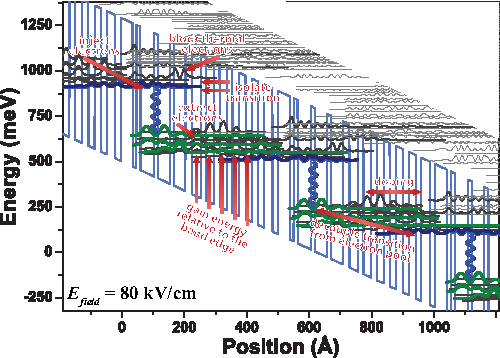
\includegraphics[width=5.5in]{Razeghi}
\caption[Conventional QC laser structure]{\tn{\textbf{Conventional QC laser structure.}}  Several of the important functions of injector regions are indicated.  This design, dating to 2004 \cite{Evans:APL:2004}, has shown the highest performance to-date from a QC laser \cite{Razeghi:SPIE:2009}.  It has a QC period length of $L_p=504~\tn{\AA}$, with 7 total injector wells.  The design energy is $\EE_{ph}=265~\tn{meV}$ ($\lambda_0=4.68~\tn{\um}$).}
\label{chpt4:Razeghi}
\end{figure}


\section{Theoretical Framework}

The motivation for minimizing injector region length is compelling.  Key among the performance parameters of high quality lasers are small threshold current densities, large slope efficiencies, and large wall-plug efficiencies.  In examining the relations for each of these performance parameters, we see that injector length plays a key role.  For example, the low temperature threshold current density is given by
\begin{equation}
 J_{th} = \delta_{ul} \frac{\epsilon_0 \lambda_0 n_\textit{eff}}{4 \pi q} \: \frac{\alpha_m + \alpha_w}{\tau_{\textit{eff}} \: z_{u \ell}^2} \frac{d_{ac}}{\Gamma N_p} \text{~.}
\end{equation}
%where $\delta_{ul}$ is the full-width-at-half-maximum (FWHM) of the gain spectrum, $\epsilon_0$ is the permittivity of free space, $\lambda_0$ is the free space wavelength, $n_\textit{eff}$ is the effective refractive index of the optical mode, $q$ is the electron charge, $\alpha_m + \alpha_w$ is the combined mirror and waveguide loss, $z_{u \ell}$ is the optical dipole matrix element between the upper and lower laser states, $L_{ac}$ is the thickness of the QC active core, $\Gamma$ is the optical confinement factor for the lasing mode, and $N_p$ is the number of QC periods in the active core.  The effective upper state lifetime $\tau_{\textit{eff}}~=~\tau_u (1-\tau_{\ell} / \tau_{u \ell})$, where $\tau_u$ is the upper laser state composite lifetime, $\tau_{\ell}$ is the lower laser state composite lifetime, and $\tau_{u \ell}$ is the transition lifetime between the upper and lower laser states.
We can see from this relation for $J_{th}$ that, for any fixed value of $L_{ac}/\Gamma$ (\emph{i.e.} fixed active core thickness and waveguide configuration), lower thresholds are achieved when more QC periods $N_p$ are ``squeezed'' into the QC stack.  Ideally then, one should shorten the overall QC period length.  But the length of the QC active region is somewhat fixed for any given emission wavelength and active region design strategy.  The only practical place to decrease the QC period length is the injector region.

As injector lengths are shortened and more QC periods are added to the active core, we can likewise expect an increase in total output power $P$.
\begin{equation}
P = N_p \frac{\EE_{ph}}{q} \eta_\textit{inj} \eta_m \frac{\tau_\textit{eff}}{\tau_\textit{eff}+\tau_{\ell}} \frac{\alpha_m}{\alpha_m + \alpha_w} (J-J_{th}) A
\end{equation}
The ``modal efficiency'' $\eta_m$ is defined as \cite{Gresch:PTL:2006}
%\begin{equation}
%\Gamma_m = \frac{\int_{x_0}^{x_0+L_{ac}} \! f^2(x) \, dx}{L_{ac}}
%\end{equation}
\begin{equation}
\eta_m = \frac{\left(\sum_i^{N_p} \Gamma_i\right)^2}{N_p \sum_i^{N_p} \Gamma_i^2}
\end{equation}
which weights the reduction of photon generation caused by (vertical) spatial hole burning. The individual, per-period confinement factor $\Gamma_i$ is effectively the ``local field coefficient'' $f^2(z)$,  where $f(z)$ is the electric field profile of the optical mode in the growth direction $z$ normalized such that $\max(f(z))=1$. %, $x_0$ and $x_0+L_{ac}$ mark the boundaries of the active core,  and we assume the refractive index over $L_{ac}$ is constant.
Two direct effects of shortened injector regions on $P$ become clear.  We have already demonstrated that shortened injectors reduce $J_{th}$, which is accompanied by a commensurate increase in $P$ for any $J > J_{th}$.  We also see a linear increase in $P$ as we fit more QC periods $N_p$ into the same mode profile (\emph{i.e.}, as $\eta_m$ remains constant).

The wall-plug efficiency $\eta_{wp}$ is yet another performance metric that should be improved by shortened injectors.  The wall-plug efficiency can be expressed as a product of constituent terms, as
\begin{equation}
\eta_{wp}= \frac{\EE_{ph}}{\EE_{ph}+\Delta_\textit{inj}+\frac{I R_\textit{series}}{N_p}} \frac{\tau_\textit{eff}}{\tau_\textit{eff}+\tau_\ell} \frac{\alpha_m}{\alpha_m + \alpha_w} \frac{(J-J_{th})}{J} \eta_\textit{inj} \eta_m
%\eta_{wp} = \frac{1}{1+\Delta_{inj} / (\EE_{ph})} \left[ 1-\frac{\tau_\textit{trans}}{\tau_{up}} \left( \frac{\alpha_m+\alpha_w}{n_s g_c N_p} + \frac{n_\textit{therm}}{n_s} \right) \right]
\end{equation}
where $I R_\textit{series}$ is the voltage drop across the device not attributable to the active core.  Insofar as there is some series resistance $R_\textit{series}$ for the device (from top and bottom contacts, for example), increasing $N_p$ will decrease the net parasitic effect on $\eta_{wp}$.  As in output power, increasing $N_p$ also increases ``current efficiency'' for $J>J_{th}$.  %$n_s$ is the per period free carrier sheet density, $g_c$ is the modal gain cross section, $n_\textit{therm}$ is the thermal population of the lower laser state, and $\tau_\textit{trans}$ is the total time needed for an electron to traverse one QC period.  Clearly, shortening the injectors\textemdash thus gaining the ability to increase $N_p$ while keeping the mode profile constant\textemdash will increase $\eta_{wp}$.  Also, the QC period transit time $\tau_\textit{trans}$ should be affected by shortening injector length.  The transit time can be simplistically thought of as $\tau_\textit{eff} + \tau_\textit{inj}$, with $\tau_\textit{inj}$ being the time it takes an electron to transit from the lower active region states to the next upper laser state.  One might intuitively reasons that, with shorter injector regions, $\tau_\textit{inj}$ decreases, in turn increasing $\eta_{wp}$.

As a final point, a reduction in the individual QC period length $L_p=\frac{L_{ac}}{N_p}$ could ultimately lead to the ability to produce more total output power.  With maximum output power $P_{max}~\propto~J_{max}-J_{th}$, a large ``dynamic range'' in operating current is desirable.  The maximum current density $J_{max}$ a QC laser can carry before a turn-off condition is reached can be found as \cite{Sirtori:JQE:1998} \cite{Aellen:JAP:2006}
\begin{equation}
J_{max} = \frac{q n_\textit{trans}}{\tau_\textit{trans}}
\end{equation}
where $\tau_\textit{trans}$ is the total time needed for an electron to traverse one QC period and $n_\textit{trans}$ is the sheet density of electrons that participate in transport across the period.  The total number of electrons present in the system $n_s$ should equal $n_\textit{trans}+n_\textit{stationary}$, with $n_s$ being the doping sheet density and $n_\textit{stationary}$ being the sheet density of conduction band electrons that do no contribute to current transport.  The transit time $\tau_\textit{trans}$ can be simplistically thought of as comprising the active region transit time and the injector region transit time $\tau_\textit{inj}$.  One might intuitively reason that, with shorter injector regions, $\tau_\textit{inj}$ decreases, therefore increasing $J_{max}$.  Expressed in another way, $\tau_\textit{trans}$ relates to the differential resistance over the active core (injectors and active regions) $R_{ac}$ as
\begin{equation}
R_{ac} = \frac{1}{A} \frac{V_{appl}}{q n_\textit{trans}} \tau_\textit{trans}
\end{equation}
where $V_{appl}$ is the applied voltage.  A shorter $\tau_\textit{trans}$ and therefore lower differential resistance means the upper laser state and injector ground state can remain in resonance over a larger range in current, increasing $J_{max}$ and $P_{max}$.

%%where $\tau_\textit{trans}$ is the total time needed for an electron to traverse one QC period and $n_\textit{trans}$ is the sheet density [$\frac{\textnormal{number}}{\textnormal{area}}$] of electrons that participate in transport across the period.
%%The total number of electrons present in the system $n_s+J/q$ should equal $n_\textit{trans}+n_\textit{stationary}$, with $n_s$ being the doping sheet density and $n_\textit{stationary}$ being the sheet density of conduction band electrons that do no contribute to current transport.
%The transit time $\tau_\textit{trans}$ can be simplistically thought of as comprising the active region transit time and the injector region transit time $\tau_\textit{inj}$.  One might intuitively reason that, with shorter injector regions, $\tau_\textit{inj}$ decreases, therefore increasing $J_{max}$.  Expressed in another way, $\tau_\textit{trans}$ relates to the differential resistance over the active core $R_{ac}$ as
%\begin{equation}
%R_{ac} = \frac{1}{A} \frac{V_{appl}}{q n_s} \tau_\textit{trans}  \text{~.}
%\end{equation}
%%where $A$ is the laser device area, and $V_{appl}$ is the applied voltage.
%A shorter $\tau_\textit{trans}$ and therefore lower differential resistance means the upper laser state and injector ground state can remain aligned in resonance over a larger range in current, increasing $J_{max}$ and $P_{max}$.  In effect, $\frac{1}{\tau_\textit{trans}}$ is the size of the ``pipe'' through which electrons can flow.  The bigger the pipe (i.e. the shorter $\tau_\textit{trans}$), the more electrons one can make available to produce photons.

When designing short injector QC lasers, one becomes particularly aware of the operating field $E_\textit{field}$.  In a QC structure, $E_\textit{field}$ is simply expressed as
\begin{equation}
E_\textit{field}~=~\frac{\EE_{ph} + \Delta_{inj}}{q L_p}
\end{equation}
Thus, for a fixed emission wavelength and optimally designed $\Delta_{inj}$, $E_\textit{field}$ and QC period length $L_p$ are inversely proportional. The consequential higher operating field for shortened injector regions often results in more difficulty in designing confinement for the upper laser state---which can be counteracted by use of high band-offset strained materials---and sometimes leads to laser reliability problems.


\section{QC Laser with Three Injector Wells}

\subsection{Design and Fabrication}

\begin{figure}[tp]%
\centering%
%\vspace{0.26in}%
\subfloat[]{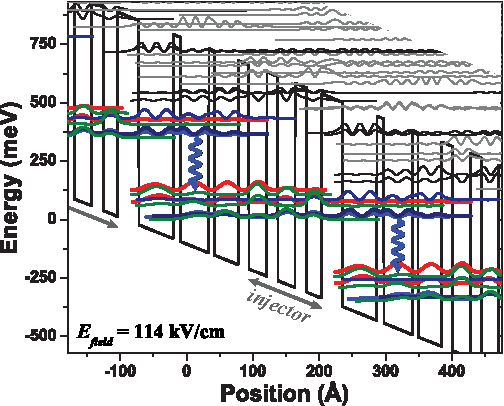
\includegraphics[width=4.25in]{80308B_114kVcm}%
\label{3well:114kVcm}}%
\\%
\subfloat[]{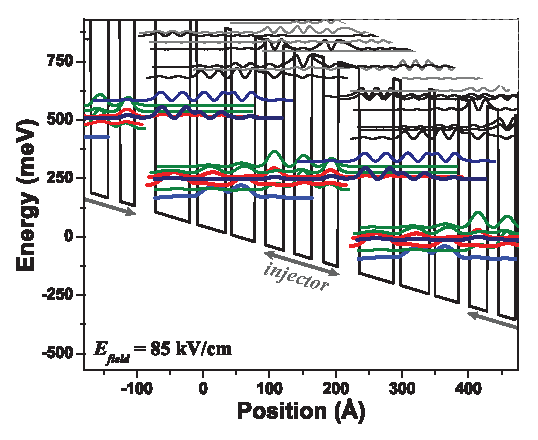
\includegraphics[width=2.8in]{80308B_85kVcm}%
\label{3well:85kVcm}}%
\hfil%
\subfloat[]{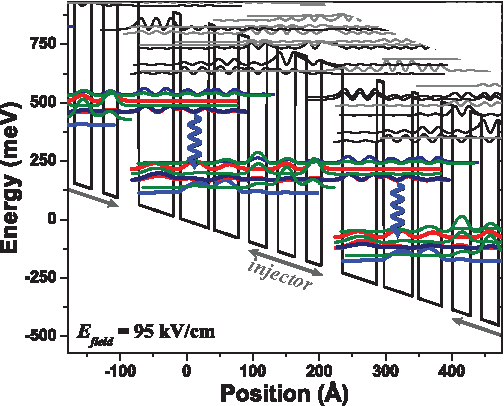
\includegraphics[width=2.8in]{80308B_95kVcm}%
\label{3well:95kVcm}}%
\caption[Energy band diagrams for the three injector well QC structure]{\tn{\textbf{Energy band diagrams for the three injector well QC structure.}}  The as-designed turn-on field is $114~\tn{kV/cm}$, shown here in \tn{(a)}.  According to EL data, current transport begins at a field of $85~\tn{kV/cm}$, shown in \tn{(b)}.  Electron transport leading to negative differential resistance is also observed starting at $95~\tn{kV/cm}$, shown in \tn{(c)}.  At 95~kV/cm the second energy level of one active region is in resonance with the down-stream upper laser state at this field.}
\label{3well:band_diagrams}
\end{figure}

We designed a QC laser consisting of six quantum wells per QC period---shown in the Fig.~\ref{3well:band_diagrams} conduction band diagram---with emission energy $\EE_{ph}$~=~239~meV ($\lambda_0$~=~5.19~$\mu$m) and energy defect $\Delta_{inj}$~=~116~meV.  With three active region wells and three injector wells, the total period length $L_p$~=~307~\AA, in contrast to $L_p$~$>$~500~\AA \ for the best conventional QC structures \cite{Lyakh:APL:2008}.  The combination of energies and period length result in a turn-on field $E_\textit{field}$~=~114~kV/cm.  The layer sequence is, in angstroms starting from the injection barrier, \textbf{32} / 52 / \textbf{10.5} / 43 / \textbf{8.5} / 36 / \textbf{16} / \underline{27} / \underline{\textbf{16.5}} / \underline{26} / \underline{\textbf{18}} / \underline{21.5}, where Al$_{0.710}$In$_{0.290}$As layers are in bold type, In$_{0.638}$Ga$_{0.362}$As layers are in plain type, and layers Si-doped $n$~=~1.0~$\times$~10$^{17}$~cm$^{-3}$ are underlined; the structure has an active core sheet density $n_s$~=~1.1~$\times$~10$^{11}$~cm$^{-2}$ per period.  At 125~kV/cm, where the upper and lower laser states are somewhat isolated, we calculate $\tau_u$~=~1.4~ps, $\tau_\ell$~=~0.5~ps, $\tau_{u\ell}$~=~5.6~ps, and $z_{u\ell}$~=~20.6~\AA, for a Figure of Merit $FoM$~= $\tau_\textit{eff} \ z_{u\ell}^2$ =~544~ps~\AA$^2$ and $FoM*$~= $\tau_\textit{eff} \ z_{u\ell}^2 \ \EE_{ph}$ =~130~ps~\AA$^2$~eV.  %At the design operating field of 114~kV/cm and using all relevant energy states, the structure has a composite Figure of Merit \cite{Franz:website:FoM} $cFoM$~=~539~ps~\AA$^2$ and $cFoM*$~=~128~ps~\AA$^2$~eV at a calculation temperature of 220~K.


The laser was grown using metal-organic vapor phase epitaxy (MOVPE) on a low doped ($n~<$~2~$\times 10^{17}$~cm$^{-3}$) InP substrate.  The QC active--injector sequence was repeated 50 times.  The QC active core was surrounded on each side by 0.12~$\mu$m~In$_{0.53}$Ga$_{0.47}$As Si-doped $n$~=~0.5~$\times~10^{17}$~cm$^{-3}$ to enhance gain region confinement factor.  Following the In$_{0.53}$Ga$_{0.47}$As confinement layer, the top cladding consisted of 2.5~$\mu$m InP Si-doped $n$~=~0.5~$\times~10^{17}$~cm$^{-3}$, 0.7~$\mu$m InP Si-doped $n$~=~80~$\times~10^{17}$~cm$^{-3}$, 0.1~$\mu$m InP Si-doped $n$~=~200~$\times~10^{17}$~cm$^{-3}$, and finally 0.06~$\mu$m In$_{0.53}$Ga$_{0.47}$As Si-doped $n$~=~500~$\times~10^{17}$~cm$^{-3}$.  Standard quantum well gradings between bulk In$_{0.53}$Ga$_{0.47}$As and InP regions were used to assist electron transport across the bulk interfaces.  For transitions from InP to In$_{0.53}$Ga$_{0.47}$As, the grading layer sequence (in angstroms) was 25 / \textbf{25} / 30 / \textbf{20} / 35 / \textbf{15} / 40 / \textbf{10} / 45 / \textbf{5}, where Al$_{0.48}$In$_{0.52}$As layers are in bold type and In$_{0.53}$Ga$_{0.47}$As layers are in plain type.

Ridge lasers with thin Au top contacts were fabricated using standard processes \cite{Franz:APL:2007}; buried heterostructure (BH) devices with InP overgrowth were likewise fabricated.  We also fabricated and tested electroluminescence (EL) mesas \cite{Franz:APL:2007} designed to suppress optical feedback in order to study spontaneous emission properties of the structure.

\subsection{Results and Discussion}

\begin{figure}[tp]%
\centering%
\subfloat[]{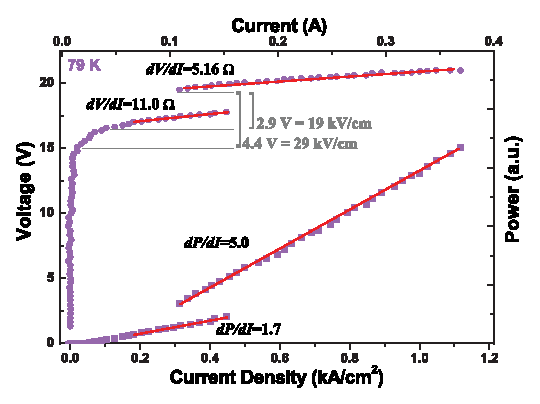
\includegraphics[width=4.25in]{3well-EL80K}%
\label{3well:EL80K}}%
\\
\subfloat[]{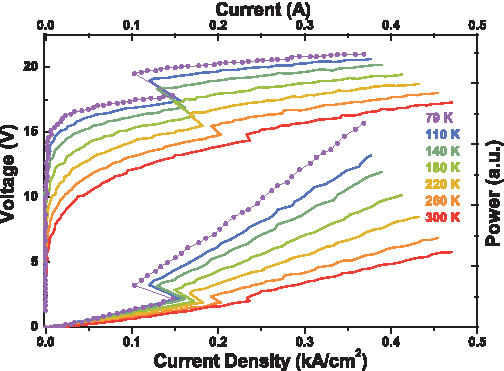
\includegraphics[width=4.25in]{3well-ELall}%
\label{3well:ELall}}%
%\vspace{0.05in}%
\caption[Three injector well EL LIV data]{\tn{\textbf{Pulsed LIV data of electroluminescence mesas for the three injector well QC structure.}}  The area of the tested device is $0.033~\tn{mm}^2$.  Pronounced negative differential resistance is seen at low temperature \tn{(a)} and persists through room temperature \tn{(b)}.}
\label{3well:EL_LIV}
\end{figure}

We examined the light--current--voltage (LIV) properties of both EL mesas and ridge lasers.  We observe a pronounced negative differential resistance (NDR) feature in all devices.  In EL mesas at a heat sink temperature $T_{sink}$~=~80~K and current densities near 0.3~kA/cm$^2$, we see a rapid 1.7~V (11~kV/cm) ``jump,'' as shown in Fig.~\ref{3well:EL80K}.  The voltage increase is accompanied by a reduction in current density of 0.13~kA/cm$^2$.  After the NDR feature, the differential resistance $dV/dI$ decreases by a factor of 2.  We also observe in the light--current (LI) data that, after the NDR feature, the radiative efficiency $dP/dI$ increases by a factor of 3.  We furthermore see from Fig.~\ref{3well:ELall} that the NDR persists through room temperature.

\begin{figure}[tp]
\centering
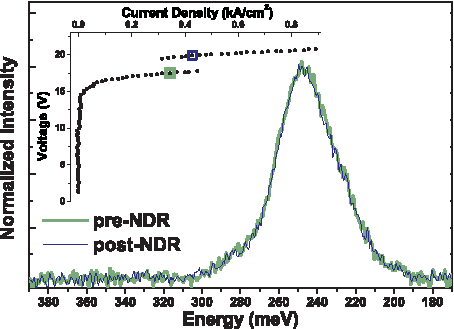
\includegraphics[width=4.25in]{3well-EL_spectra}
\caption[Comparison of EL spectra at pre- and post-NDR operating points]{\tn{\textbf{Comparison of EL spectra at pre- and post-NDR operating points.}}  The pre-NDR point, light-colored bold line, is at $J=0.34~\tn{kA/cm}^2$ and $V=17.5~\tn{V}$.  The post-NDR point, dark-colored narrow line, is at $J=0.43~\tn{kA/cm}^2$ and $V=19.9~\tn{V}$.  We observe no spectral distinction between the two operating points.  The spectral resolution of the data is $1~\tn{meV}$.}
\label{3well:EL_spectra}
\end{figure}


\begin{figure}[tp]
\centering
\subfloat[]{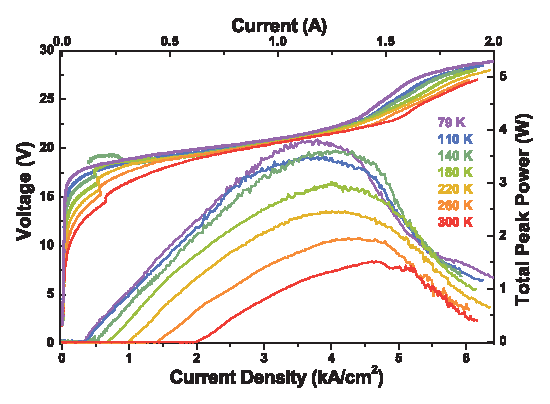
\includegraphics[width=4.25in]{3well-lasing}%
\label{3well:lasing}}%
\\
\subfloat[]{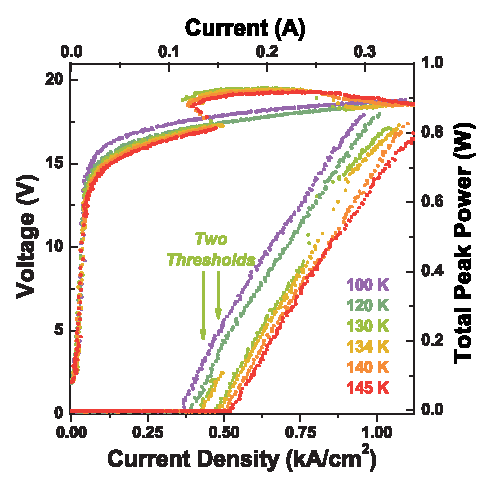
\includegraphics[width=2.8in]{3well-lasing_zoom}%
\label{3well:lasing_zoom}}%
\hfil
\subfloat[]{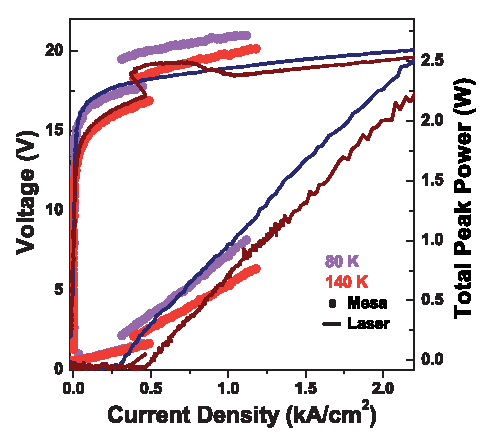
\includegraphics[width=2.8in]{3well-EL_lasing}%
\label{3well:EL_lasing}}%
\caption[Three injector well LIV]{\tn{\textbf{Three injector well LIV.}} A representative ridge laser device, $10.4~\tn{\um}\times3~\tn{mm}$.  As seen in \tn{(a)}, negative differential resistance (NDR) is observed, but only at elevated temperatures.  From \tn{(b)}, we see that the NDR appears only for $J_{th}>J_{NDR}$, \emph{i.e.} here for $T_{sink}\geq130~\tn{K}$.  Because of the NDR, we observe two thresholds for $T_{sink}=130~\tn{K}$ and slightly above.  The comparison of LIV data from this laser device and EL data from Fig.~\ref{3well:ELall}, as in \tn{(c)}, shows the effect of cavity photon density on the current--voltage behavior.}
\label{3well:lasing_LIV}
\end{figure}

\begin{figure}[tp]
\centering
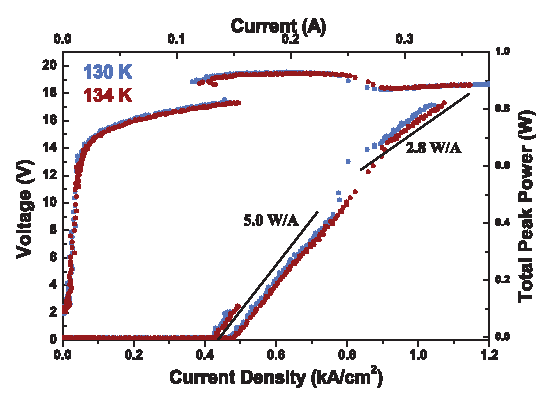
\includegraphics[width=4.25in]{3well-LIV_slopes}
\caption[Three injector well LIV near $T_{sink}=130~\tn{K}$]{\tn{\textbf{Three injector well LIV near \textbf{\textit{T\sub{\textbf{sink}}}=130~\tn{\textbf{K}}}.}}  Different slope efficiencies are observed before and after the band configuration that results from the presence of stimulated emission.  No observable change in slope efficiency is observed before and after the NDR point.}
\label{3well:LIV_slopes}
\end{figure}

The NDR can be understood in that the two operating states---before the NDR feature and after---represent two different energy band configurations.  At $T_{sink}=80$~K, the difference in turn-on of the two current paths is 2.9~V (19~kV/cm).  Associating the current path in operation after the NDR feature with the band alignment at the design field of 114~kV/cm, the first current path operates with turn-on at 95 kV/cm.  The energy diagram at 95 kV/cm, plotted in Fig.~\ref{3well:95kVcm}, elucidates a process of electron transport across the injector region after just a single phonon transition from the lower laser state.  In this case, $\Delta_{inj}=49$~meV, rather than the 116~meV at 114~kV/cm.

Interestingly, this is strong evidence of current flow and light generation with the lowest state of one active region significantly below the upper laser state of the next down-stream active region.  At the lower field of 95~kV/cm in Fig.~\ref{3well:95kVcm}, most of the dopant electrons $n_s$ are ``trapped'' in the lowest active region state (\emph{i.e.} $n_\textit{stationary}\approx n_s$).  In contrast, at $E_\textit{field}=114$~kV/cm, $n_\textit{trans}\approx n_s$.  %Therefore, the only contribution to $n_\textit{trans}$ is the injected current $J/q$, yielding a substantially smaller $J_{max}$ at this band alignment than at $E_\textit{field}=114$~kV/cm where $n_\textit{trans}\approx n_s$.
The NDR can thus be interpreted as the existence of two different values of $J_{max}$: one for the 95~kV/cm band alignment, and a second, larger $J_{max}$ for the 114~kV/cm band alignment.

EL spectra collected at pre- and post-NDR points, as in Fig.~\ref{3well:EL_spectra}, are absent any discernable spectral changes between the two operating points.  We thus conclude that the upper and lower energy states of the optical transition remain the same between the two operating points.  The field re-alignment changes only the configuration of the injector states relative to the active region states.

\medskip

The data become all the more interesting for laser devices, \emph{i.e.} with the inclusion of stimulated emission in the overall device behavior. Figure~\ref{3well:lasing} shows that no NDR is observed in the current--voltage (IV) data at 80~K.  Rather, the NDR only appears at temperatures near and above 140~K.  Figure~\ref{3well:lasing_zoom} shows the onset of NDR behavior with greater temperature resolution.  Here, we see the NDR feature appear at 130~K, the first temperature where threshold current density is greater than the current density at which the NDR occurs ($J_{th}~>~J_{NDR}$).  Apparently, it is the presence of cavity photons (stimulated emission) that prevents the observation of NDR and locks the laser into the pre-NDR band configuration for $T_{sink}~<$~130~K.  Also of note is that the laser exhibits two thresholds for $T_{sink}$~=~130~K and slightly above.  The two thresholds directly result from the NDR---that is, the decrease in pumping current as the energy level configuration re-aligns at the higher field.

Perhaps even more surprising, for $T_{sink}$ corresponding to $J_{th}~>~J_{NDR}$, increasing cavity photon density actively ``pulls down'' the operating voltage.  Effectively, the internal electric field decreases, returning the band configuration to the pre-NDR state.  This, in fact, is a second form of NDR, where voltage decreases with increasing current, rather than the more typically thought-of NDR where current decreases with increasing voltage. The feature can plainly be seen in Fig.~\ref{3well:EL_lasing}, where we compare LIV data from mesa and laser devices at $T_{sink}$~=~80~K and 140~K.

The behavior of these two NDR features can be explained by considering contributions to the total per period transport rate $\frac{1}{\tau_\textit{trans}}$.  We can simplify the total carrier transit time through a QC period $\tau_\textit{trans}$ as being the sum of active region and injector region transit times due to non-radiative processes such as phonon scattering---respectively $\tau_\textit{act}$ and $\tau_\textit{inj}$---and including a term $\tau_\textit{stim}$ that accounts for photon-assisted transport due to stimulated emission.  The stimulated emission term effectively decreases the active region transit time.%\footnote{$\tau_\textit{stim}$ is not necessarily equal to $\tau_\textit{eff}$}
\begin{equation}
\tau_\textit{trans} = \left(\tau_\textit{act}^{-1} + \tau_\textit{stim}^{-1} \right)^{-1} + \tau_\textit{inj}
\end{equation}
%the transit time through the active region due to stimulated emission $\frac{1}{\tau_\textit{stim}}$ along with the rate of transport through the active region $\frac{1}{\tau_\textit{act}}$ and injector region $\frac{1}{\tau_\textit{inj}}$ due to LO phonons and other non-radiative scattering.
%\begin{subequations}
%\begin{gather}
%\frac{1}{\tau_\textit{trans}}=\frac{1}{\tau_\textit{act,stim}}+\frac{1}{\tau_\textit{inj}}\\
%\frac{1}{\tau_\textit{act,stim}}=\frac{1}{\tau_\textit{act}}+\frac{1}{\tau_\textit{stim}}
%\end{gather}
%\end{subequations}
Here, $\tau_\textit{act}$ and $\tau_\textit{stim}$ are grouped in recognition that active region transport may be either by stimulated emission and/or non-radiative scattering.  To explain the first NDR feature, where the temperature dependence of $J_{th}$ affects the presence of this NDR, we return to our consideration of $J_{max}$.  Stimulated emission significantly extends $J_{max}$, especially if the total non-radiative transport time is dominated by $\tau_\textit{act}$ (due to the long lifetime of the upper laser state) in the absence of stimulated emission.  Thus, for temperatures below 130~K where no NDR is observed, $J_{max}(E_\textit{field}=95~\textnormal{kV/cm})$ includes stimulated emission and is therefore large.  For temperatures at and above 130~K where we see NDR, $J_{max}(E_\textit{field}=95~\textnormal{kV/cm})$ is smaller since $J_{th}<J_{max}$.

To explain the second NDR feature, where voltage decreases with increasing current for $T_\textit{sink}\geq130$~K, we again look to the effect of stimulated emission on $\frac{1}{\tau_\textit{trans}}$ and $J_{max}$.  Specifically, this behavior can be understood with the insight that $J_{max}$ \emph{changes} with the presence of stimulated emission, and the assumption that, faced with two transport options, the device will naturally operate in the configuration that minimizes $\tau_\textit{trans}$.  For $T_\textit{sink}\geq130$~K, $J_{max}(E_\textit{field}=114~\textnormal{kV/cm})>J_{th}$, but, due to the presence of stimulated emission, $J_{max}(E_\textit{field}=95~\textnormal{kV/cm})$ is also greater than $J_{th}$ \emph{once lasing has been established}.  Now, with two available transport paths, the laser selects the path that minimizes transport time.  %is it transport time or energy?  It's the same here, but what if it wasn't?
%At 114~kV/cm and only considering LO phonon scattering, we calculate the injector transport time to be 0.7~ps; at 95~kV/cm---where fewer states exist between successive lower and upper laser levels---the injector transport time is 0.6~ps.  The difference is expected to be even larger with the inclusion of resonant tunneling.
Thus, the presence of stimulated emission causes the laser to revert back to the lower field configuration.%Thus, as stimulated emission reduces the upper laser state lifetime, the introduction of such a non-linear shift in the electron distribution profile creates a configuration where the pre-NDR transport path is preferred.
%In a lasing device, with stimulated emission contributing to $\frac{1}{\tau_\textit{trans}}$, the injector transport rate becomes dominant.
%Furthermore, the transport paths are different in the spontaneous emission case of EL mesas and in the case of a laser device.  Electrons non-radiatively scatter into all lower active region states versus the case where all electrons pass are deposited in the lower laser state.

%, $\frac{1}{\tau_\textit{trans}}$ is dominated by $\tau_\textit{act}$ due to the relatively large upper laser state lifetime.

After the second NDR feature, we observe a marked decrease in slope efficiency.  In Fig.~\ref{3well:LIV_slopes}, we see that the slope efficiency for the low field band configuration (Fig.~\ref{3well:95kVcm}) is nearly half that of the high field configuration (Fig.~\ref{3well:114kVcm}): 2.8 vs.\ 5.0~W/A, respectively.  This discrepancy is at least consistent with the factor of 3 observed in the EL case (Fig.~\ref{3well:EL_LIV}).  Although the exact origin is unclear, we can narrow the source of the difference down to either injection efficiency into the upper laser state or the laser transition efficiency, since $\frac{d P}{dI}\propto \eta_\textit{inj} \frac{\tau_\textit{eff}}{\tau_\textit{eff}+\tau_{\ell}}$, and no other terms in $\frac{d P}{dI}$ change with a change in band structure configuration alone.


\subsection{Device Performance}

Figures \ref{3well:spectra_79K}, \ref{3well:spectra_146K}, and \ref{3well:spectra_302K} show laser spectra at $T_{sink}=79$, 146, and 302~K, respectively.  Shown with each set of data is an LIV plot, with each LIV point corresponding to a spectral measurement.  The NDR feature is clearly seen in the $T_{sink}=146$~K LIV data, but no discernable spectral feature can be distinctly correlated with the NDR.  As shown in Fig.~\ref{3well:lasing_spectrum}, a standard red-shift is seen with increasing temperature: $\lambda_0\approx5.1$~\um\ for $T_{sink}=79$~K and $\lambda_0\approx5.4$~\um\ at room temperature.

\begin{figure}[tp]
\centering
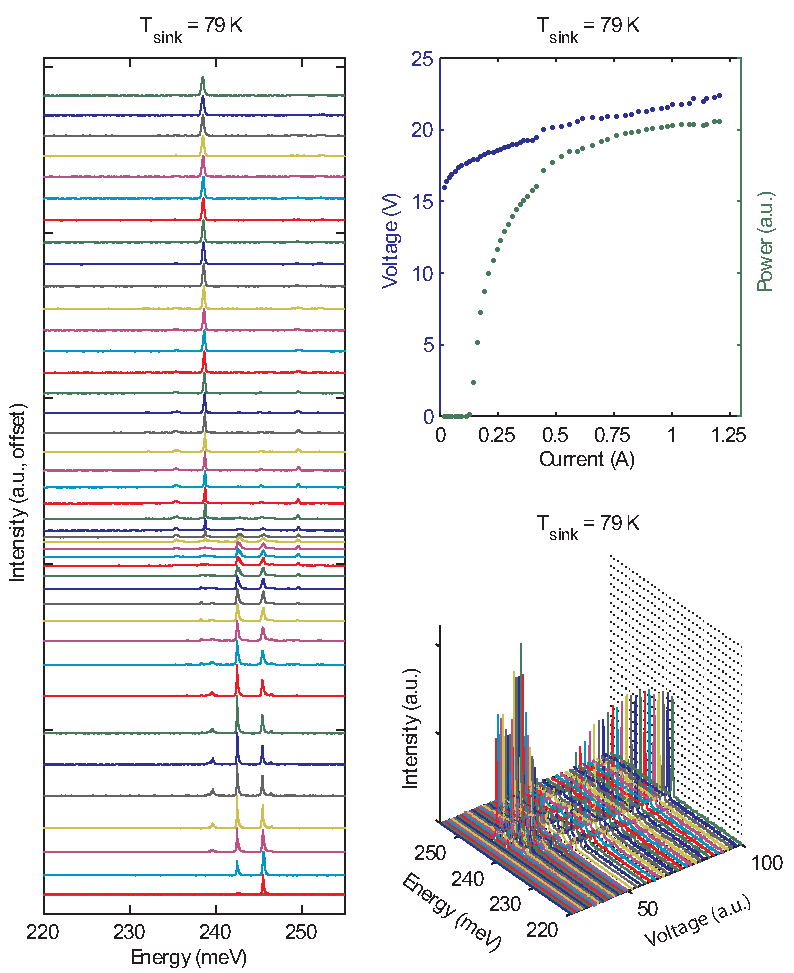
\includegraphics[width=6in]{3well-spectra_79K}
\caption[Spectra for the 3 injector well laser at $T_{sink}=79~\tn{K}$]{\textnormal{\textbf{Spectra for the 3 injector well laser at \textit{T}\sub{\textit{sink}}~=~79~K.}}  The device size was $10.4~\tn{\um} \times 3~\tn{mm}$ pulsed at $80~\tn{kHz}$ with a $100~\tn{ns}$ current pulse.  Each point in the LIV (top--right) has one corresponding spectra in the left and bottom--right plots.}
\label{3well:spectra_79K}
\end{figure}

\begin{figure}[tp]
\centering
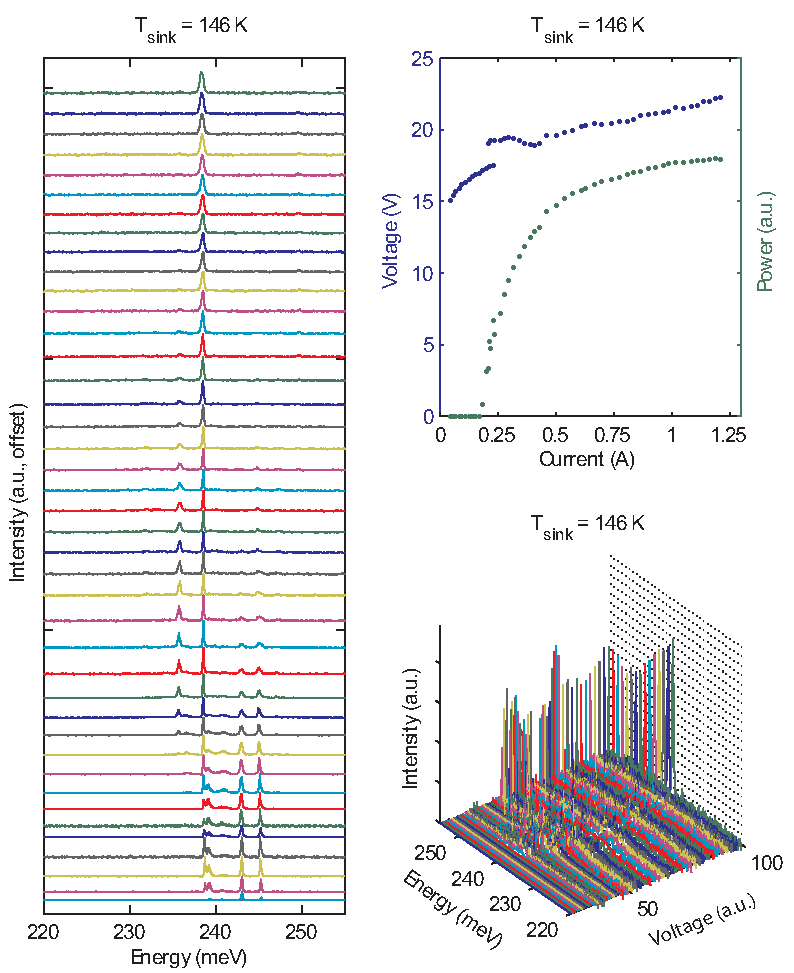
\includegraphics[width=6in]{3well-spectra_146K}
\caption[Spectra for the 3 injector well laser at $T_{sink}=146~\tn{K}$]{\textnormal{\textbf{Spectra for the 3 injector well laser at \textit{T}\sub{\textit{sink}}~=~146~K.}}  The device size was $10.4~\tn{\um} \times 3~\tn{mm}$ pulsed at $80~\tn{kHz}$ with a $100~\tn{ns}$ current pulse.  Each point in the LIV (top--right) has one corresponding spectra in the left and bottom--right plots.}
\label{3well:spectra_146K}
\end{figure}

\begin{figure}[tp]
\centering
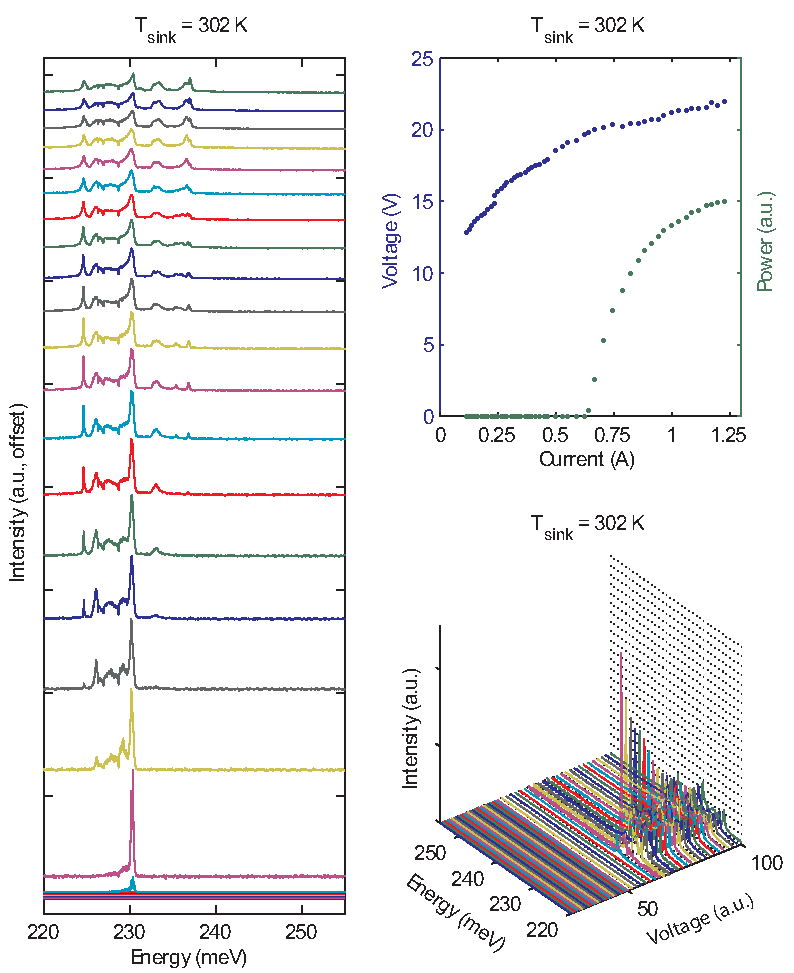
\includegraphics[width=6in]{3well-spectra_302K}
\caption[Spectra for the 3 injector well laser at $T_{sink}=302~\tn{K}$]{\textnormal{\textbf{Spectra for the 3 injector well laser at \textit{T}\sub{\textit{sink}}~=~302~K.}}  The device size was $10.4~\tn{\um} \times 3~\tn{mm}$ pulsed at $80~\tn{kHz}$ with a $100~\tn{ns}$ current pulse.  Each point in the LIV (top--right) has one corresponding spectra in the left and bottom--right plots.}
\label{3well:spectra_302K}
\end{figure}

\begin{figure}[tp]%
\centering%
\subfloat[]{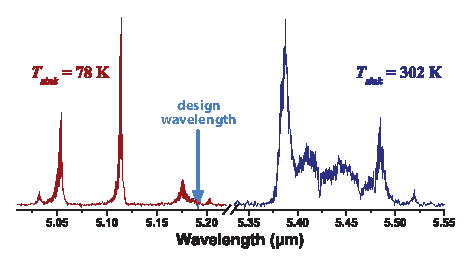
\includegraphics[width=3.25in]{3well-laser-spectrum}%
\label{3well:lasing_spectrum}}%
\\%
\vspace*{-0.1in}%
\subfloat[]{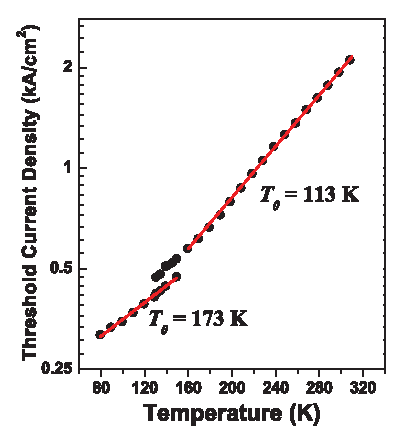
\includegraphics[width=2.75in]{3well-T0}%
\label{3well:T0}}%
\hfil%
\subfloat[]{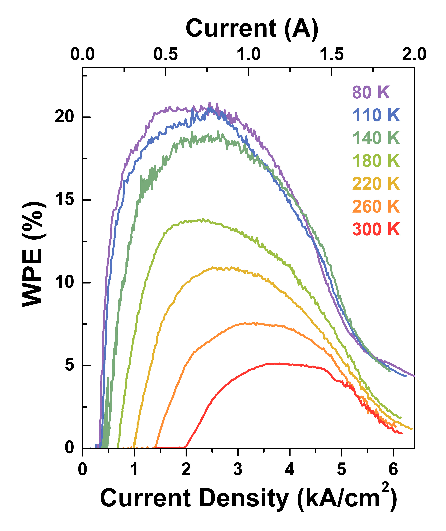
\includegraphics[width=2.75in]{3well-WPE_tifeps}%
\label{3well:WPE}}%
\caption[Performance data for the three injector well structure]{\tn{\textbf{Performance data for the three injector well structure.}} \tn{(a)} Representative normalized spectra of the three injector well structure for $T_{sink}=78~\tn{K}$ and $302~\tn{K}$ near threshold.  Characteristic temperature $T_0$ \tn{(b)} and pulsed wall-plug efficiency \tn{(c)} for a $10.4~\tn{\um}\times3~\tn{mm}$ ridge laser device.}%
\label{3well:performance}%
\end{figure}

For the ridge laser device described by the Fig. \ref{3well:lasing_LIV} data, pulsed total output power peaks at 3.8~W at 80~K, while room temperature output power is 1.5~W.  Threshold current density is 313~A/cm$^2$ at 80~K, and reaches 2.0~kA/cm$^2$ at room temperature. Figure \ref{3well:T0} explains this result, with the rather low characteristic temperature $T_0$~=~113~K for $T_{sink}$ where $J_{th}~>~J_{NDR}$.  However, for $T_{sink}$ where $J_{th}~<~J_{NDR}$, $T_0$ is much higher at 173~K.  Wall-plug efficiency---as shown in Fig.~\ref{3well:WPE}---peaks at 20.5\% for $T_{sink}$~=~80~K and 5.1\% at 300~K.

%\begin{figure*}[!t]%
%\centering%
%\subfloat[]{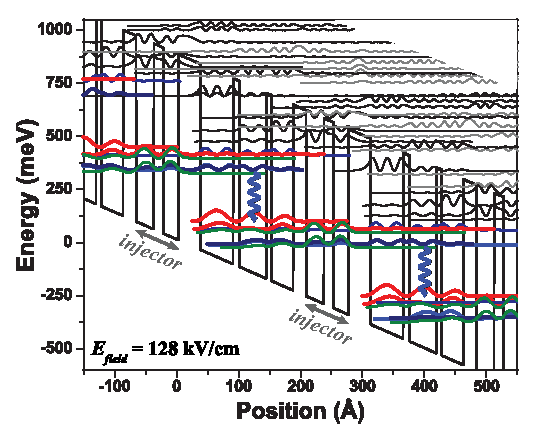
\includegraphics[width=3.25in]{80308A_128kVcm}%
%\label{2well:128kVcm}}%
%\\%
%%\vspace*{-0.1in}%
%\subfloat[]{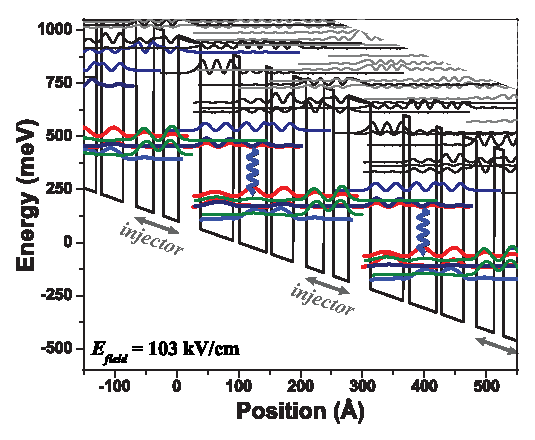
\includegraphics[width=3.25in]{80308A_103kVcm}%
%\label{2well:103kVcm}}%
%\hfil%
%\subfloat[]{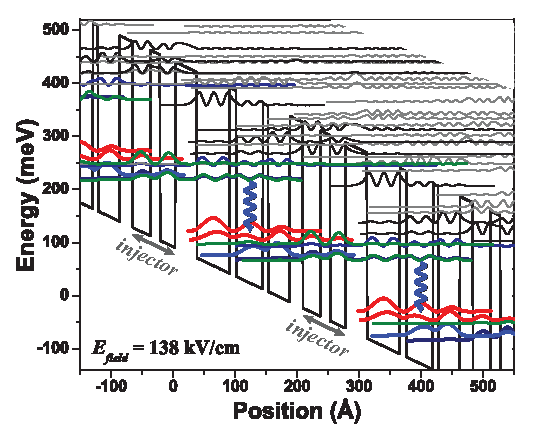
\includegraphics[width=3.25in]{80308A_138kVcm}%
%\label{2well:138kVcm}}%
%\caption{QC structure with two injector wells and three active region wells.  The designed turn-on field is 128~kV/cm, shown in (a).  NDR is observed in this structure at $E_\textit{field}$~=~103~kV/cm, shown in (b).  Also, an increase in differential resistance is seen in device data consistent with a re-configuration of the band alignment where the upper laser state is in resonance with the injector ground state, as in (c), near $E_\textit{field}$~=~138~kV/cm.}
%\label{2well:band_diagrams}
%\end{figure*}

\section{QC Laser with Two Injector Wells}

\subsection{Design and Fabrication}

\begin{figure}[tp]%
\centering%
\subfloat[]{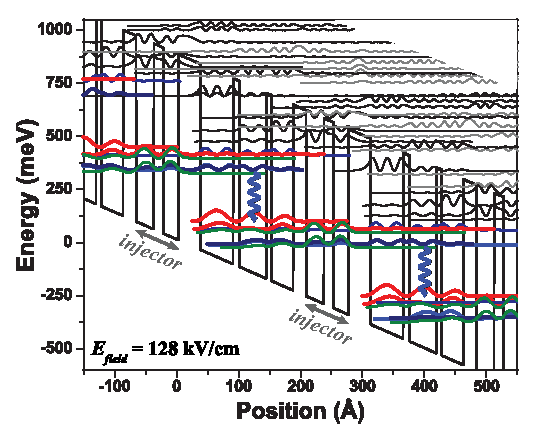
\includegraphics[width=4.25in]{80308A_128kVcm}%
\label{2well:128kVcm}}%
\\%
\subfloat[]{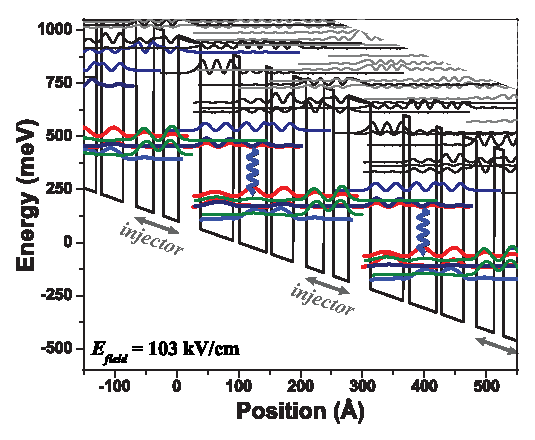
\includegraphics[width=2.8in]{80308A_103kVcm}%
\label{2well:103kVcm}}%
\hfil%
%\vspace*{-0.1in}%
\subfloat[]{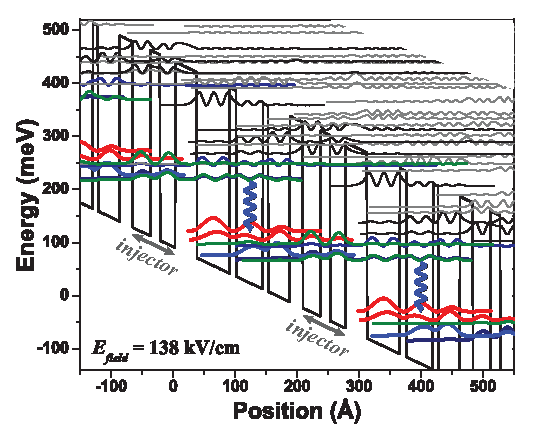
\includegraphics[width=2.8in]{80308A_138kVcm}%
\label{2well:138kVcm}}%
\caption[Energy band diagrams for the two injector well QC structure]{\tn{\textbf{QC structure with two injector wells and three active region wells.}}  The designed turn-on field is $128~\tn{kV/cm}$, shown here in \tn{(a)}.  NDR is observed in this structure at $E_\textit{field}=103~\tn{kV/cm}$, shown in \tn{(b)}.  Also, an increase in differential resistance is seen in device data consistent with a re-configuration of the band alignment where the upper laser state is in resonance with the injector ground state, as in \tn{(c)}, near $E_\textit{field}=138~\tn{kV/cm}$.}
\label{2well:band_diagrams}
\end{figure}

To further test such short injector structures, we designed a second laser with only two injector wells and three active region wells.  Besides the removal of one injector well, the two laser designs are otherwise similar.  The emission energy was designed to be $\EE_{ph}$~=~241~meV ($\lambda_0$~=~5.14~$\mu$m) and energy defect designed to be $\Delta_{inj}$~=~107~meV.  The total QC period length $L_p$~=~274.5~\AA, for a design field $E_\textit{field}$~=~128~kV/cm.  As shown in the Fig.~\ref{2well:band_diagrams} conduction band diagram, the layer sequence is, in angstroms starting from the injection barrier, \textbf{35} / 53 / \textbf{10.5} / 43 / \textbf{8.5} / 35 / \textbf{21} / \underline{28.5} / \underline{\textbf{15.5}} / \underline{24.5}, where Al$_{0.710}$In$_{0.290}$As layers are in bold type, In$_{0.638}$Ga$_{0.362}$As layers are in plain type, and layers Si-doped $n$~=~1.4~$\times$~10$^{17}$~cm$^{-3}$ are underlined; the structure has an active core sheet density $n_s$~=~0.96~$\times$~10$^{11}$~cm$^{-2}$.  At 132~kV/cm, with the upper laser state somewhat isolated from the injector region states, we calculate $\tau_u$~=~1.41~ps, $\tau_\ell$~=~0.23~ps, $\tau_{u\ell}$~=~4.55~ps, and $z_{u\ell}$~=~20.1~\AA, for a Figure of Merit $FoM$~=~542~ps~\AA$^2$ and $FoM*$~=~131~ps~\AA$^2$~eV.  %At the designed operating field of 128~kV/cm and using all relevant energy states, the structure has a composite Figure of Merit $cFoM$~=~659~ps~\AA$^2$ and $cFoM*$~=~159~ps~\AA$^2$~eV at a calculation temperature of 220~K.

The laser was grown by MOVPE with a waveguide structure identical to that described in the previous section.  Fabrication and processing were also similar.


\subsection{Results and Discussion}

Similar to the three well injector design reported in the previous section, LIV data for this design also show NDR, as seen in Fig.~\ref{2well:EL_LIV} for an EL mesa; in this case though, it is much less pronounced.  Following the analysis of the previous section, the NDR appears 3.6~V (26~kV/cm) below the designed turn-on voltage.  In this design, we calculate that the upper laser state and the second active region state of the up-stream active region mix at $E_\textit{field}$~=~103~kV/cm; here, the difference between the field at which these states align and the designed turn-on field---25~kV/cm---is in excellent agreement with the data.  However, the states mix to a much less extent, which is consistent with the lower current change associated with the NDR feature.

\begin{figure}[tp]
\centering
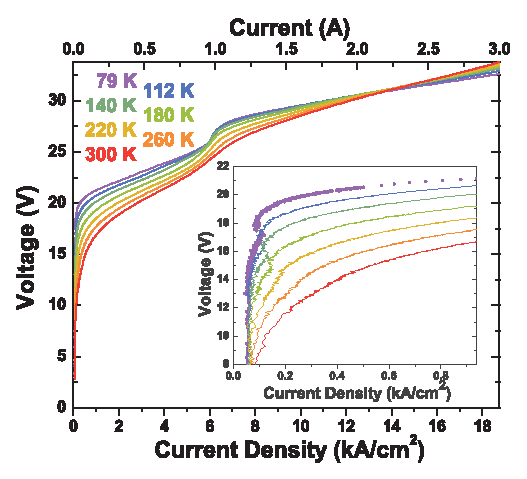
\includegraphics[width=4in]{2well-EL_LIV}
\caption[LIV for a two injector well EL sample]{\tn{\textbf{LIV for a two injector well EL sample.}} NDR is also seen in the two injector well design, but it is much less pronounced than in the three injector well design.  Here, we see small NDR for a $0.016~\tn{mm}^2$ EL mesa.}
\label{2well:EL_LIV}
\end{figure}

The two injector well design shows other characteristic features in the LIV data.  For example, in Fig.~\ref{2well:laser_LIV} we see two physically separate mechanisms that limit light output.  For an applied 20~V, we see an increase in differential resistance; the feature is roughly independent of temperature, and it corresponds to a drop in slope efficiency.  A second increase in differential resistance is observed, this time at a constant current density of about 7~kA/cm$^2$ (independent of temperature).  Again, this feature generally corresponds to a decrease in output power.  That the first effect appears with constant applied field and the second appears with constant current density is telling of the physical origins.  The constant-current feature is the ``turn-off'' most commonly seen in QC lasers, where a maximum current density is reached based on the intrinsic transit times and the finite amount of doping $n_s$ of the QC structure \cite{Aellen:JAP:2006}.

The constant-voltage turn-off feature in Fig.~\ref{2well:laser_LIV} is not as commonly observed.  One explanation for this feature arises from examining the injector region configuration relative to the active region at different fields.  At $T_{sink}=79$~K, the difference between the turn-on voltage of the device and this constant-voltage turn-off is about 2.1~V (15~kV/cm).  Our laser was intentionally designed for the lowest state of one active region to be in resonance with the upper laser state of the adjacent down-stream active region at threshold, providing efficient transport between active regions and thus decreasing $\tau_\textit{inj}$.  In this design, these levels are in full resonance when $E_\textit{field}$~=~128~kV/cm.  However, because of the spatial separation of these two states, they remain strongly coupled over only a small field range.  At $E_\textit{field}$~=~128~kV/cm, the lowest injector state is below these two aligned states; increasing the field to 138~kV/cm puts the lowest injector state and the upper laser state in full resonance.  This secondary field alignment and electron path is conceivably slower, as electrons have to travel through an additional state, increasing the differential resistance.  The increase in differential resistance observed at constant applied field with variations in temperature may thus arise from these two injector region alignments.  The successful operation of both these band alignments is further evidence that electrons can directly tunnel from one active region to the next---in effect, ballistic transport---in these short injector structures.

\begin{figure}[tp]%
\centering%
\subfloat[]{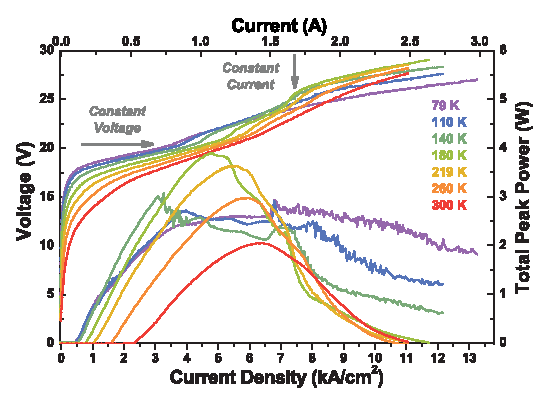
\includegraphics[width=4.25in]{2well-laser_a529ZB}%
\label{2well:laser_a529ZB}}%
\\%
\subfloat[]{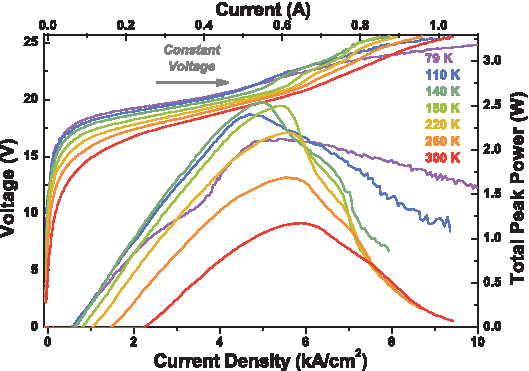
\includegraphics[width=4.25in]{2well-laser_a529ZF}%
\label{2well:laser_a529ZF}}%
\caption[Pulsed LIV data for the two injector well structure (I)]{\tn{\textbf{Pulsed LIV data for the two injector well structure (I).}} Panel \tn{(a)} is for a $7.5~\tn{\um}\times3~\tn{mm}$ BH laser and \tn{(b)} is for a $5.5~\tn{\um}\times2~\tn{mm}$ BH laser.  Two ``turn-off'' features are seen, one occurring with constant voltage and one with constant current.  Pulse instabilities are also evident at lower temperatures.  Because of these instabilities, output power is highest at elevated temperatures.}
\label{2well:laser_LIV}
\end{figure}

\begin{figure}[tp]%
\centering%
\subfloat[]{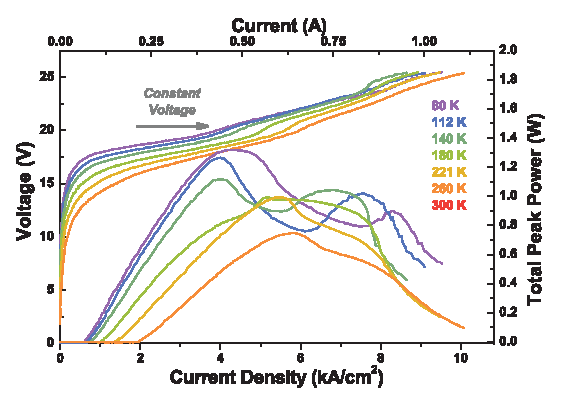
\includegraphics[width=4.25in]{2well-laser_a529ZA}%
\label{2well:laser_a529ZA}}%
\\%
\subfloat[]{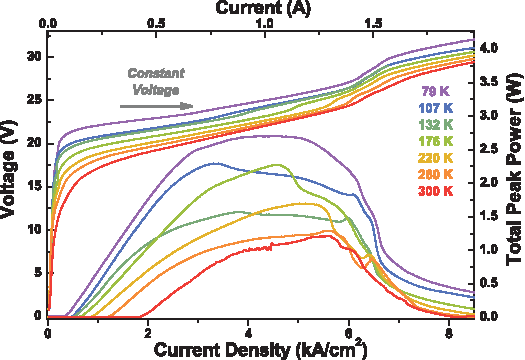
\includegraphics[width=4.25in]{2well-laser_a529ADb}%
\label{2well:laser_a529ADb}}%
\caption[Pulsed LIV data for the two injector well structure (II)]{\tn{\textbf{Pulsed LIV data for the two injector well structure (II).}} Panel \tn{(a)} is for a $5.5~\tn{\um}\times2~\tn{mm}$ BH laser and \tn{(b)} is for a $13~\tn{\um}\times3~\tn{mm}$ ridge laser.  Again, two ``turn-off'' features are evident, one occurring with constant voltage and one with constant current.}
\label{2well:laser_LIV2}
\end{figure}


Yet another interesting feature is seen in the Fig.~\ref{2well:laser_LIV} LIV characteristics.  Rather than peak output at the lowest temperatures, these lasers have peak output at elevated temperatures (180~K in this device), while highly unstable pulse behavior at lower temperatures limits average output power. The time evolution of the light pulse over the 100~ns period also indicates highly irregular behavior, with pulse-to-pulse variations on the order of 100~mW at low temperatures. These pulse instabilities are damped with increasing temperature, and they disappear around 140~K.

%With these extremely short period structures (here, five quantum wells total per period), we might expect to recover more "classical" superlattice behavior.

In QC structures, electric field profiles are largely assumed to be homogenous when the doping density is low, or periodic but stable when the doping density is higher. However, charge instabilities have long been known to exist in superlattice structures \cite{Leo:book:2006}. Intuitively, charge instabilities can result when local disruptions of the charge density locally perturb the field, leading to electric field domains. The highly nonlinear event of lasing onset is expected to exacerbate this instability, and in these minimalized QC structures, these instabilities are now more apparent.

Both of the previous features---constant-voltage turn-off and pulse instabilities---result from the highly discrete nature of the individual quantum states in our structure.  In actuality, we have composed a QC structure out of only six relevant states: a ground state for each of the five quantum wells in the QC period and one quantum well first-excited state that is the upper laser state.  Having only six states spread across $\Delta_\textit{inj}$~=~107 meV is unusual for QC structures; a comparable conventional design with a four well active region and seven injector wells would have 12 states spread across the same $\Delta_\textit{inj}$. In this situation, we see the effect of the highly discrete injector region states; the positioning of individual states matters more than ever.

\subsection{Device Performance}

\begin{figure}[tp]
\centering
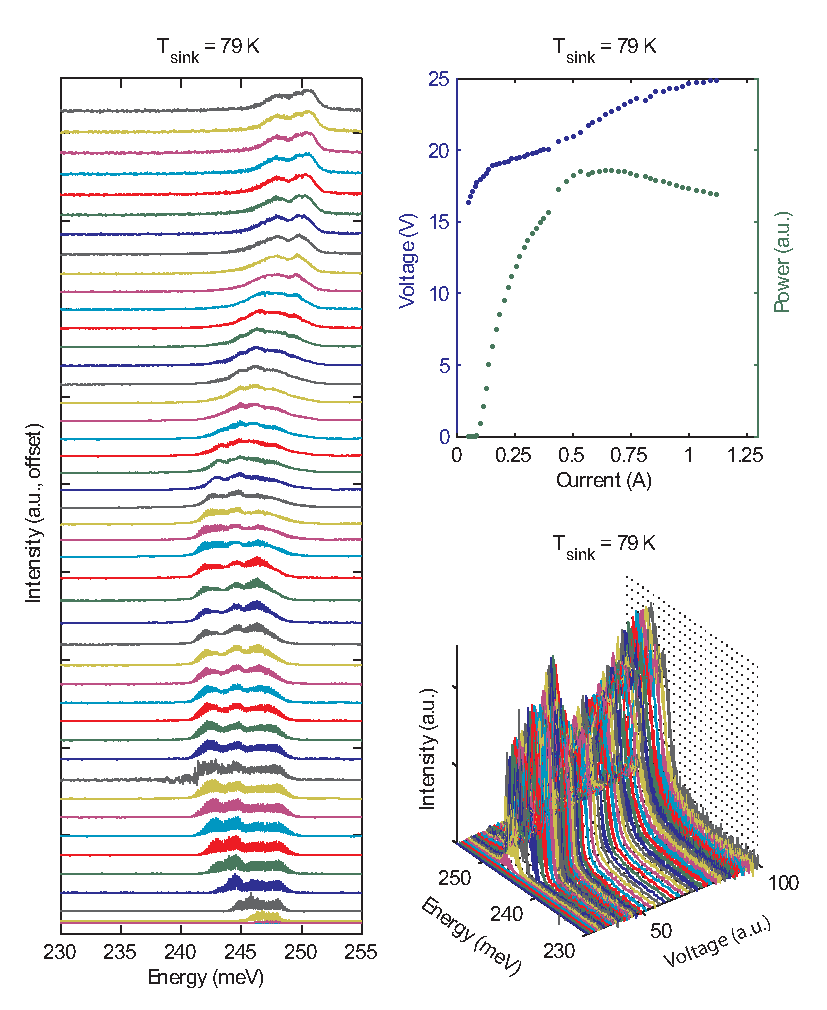
\includegraphics[width=6in]{2well-spectra_79K}
\caption[Spectra for the 2 injector well laser at $T_{sink}=79~\tn{K}$]{\textnormal{\textbf{Spectra for the 2 injector well laser at \textit{T}\sub{\textit{sink}}~=~79~K.}}  The device size was $5.5~\tn{\um} \times 2~\tn{mm}$ pulsed at $80~\tn{kHz}$ with a $100~\tn{ns}$ current pulse, and corresponds to the LIV data in Fig.~\ref{2well:laser_a529ZF}.  Each point in the LIV (top--right) has one corresponding spectra in the left and bottom--right plots.}
\label{2well:spectra_79K}
\end{figure}

\begin{figure}[tp]
\centering
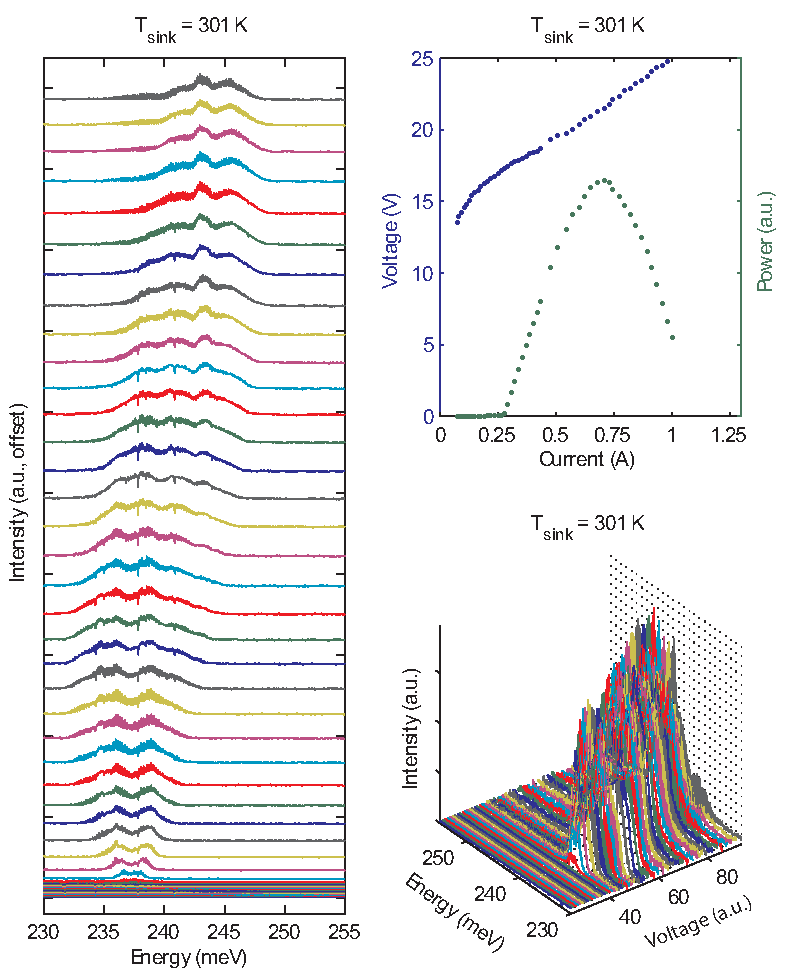
\includegraphics[width=6in]{2well-spectra_301K}
\caption[Spectra for the 2 injector well laser at $T_{sink}=301~\tn{K}$]{\textnormal{\textbf{Spectra for the 2 injector well laser at \textit{T}\sub{\textit{sink}}~=~301~K.}}  The device size was $5.5~\tn{\um} \times 2~\tn{mm}$ pulsed at $80~\tn{kHz}$ with a $100~\tn{ns}$ current pulse, and corresponds to the LIV data in Fig.~\ref{2well:laser_a529ZF}.  Each point in the LIV (top--right) has one corresponding spectra in the left and bottom--right plots.}
\label{2well:spectra_301K}
\end{figure}

Figures \ref{2well:spectra_79K} and \ref{2well:spectra_301K} show laser spectra at $T_{sink}=79$ and 301~K, respectively.  Shown with each set of data is an LIV plot, with each LIV point corresponding to a spectral measurement.  As shown in Fig.~\ref{2well:lasing_spectrum}, a standard red-shift is seen with increasing temperature: $\lambda_0\approx5.0$~\um\ for $T_{sink}=79$~K and at $\lambda_0\approx5.2$~\um\ at room temperature.

\begin{figure}[tp]%
\centering%
\subfloat[]{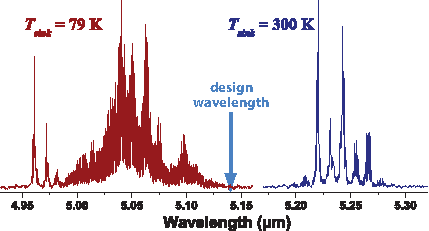
\includegraphics[width=3.25in]{2well-laser-spectrum}%
\label{2well:lasing_spectrum}}%
\\%
\vspace*{-0.1in}%
\subfloat[]{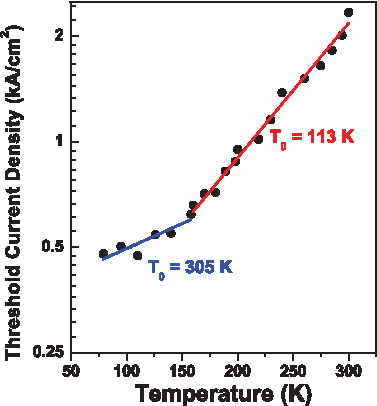
\includegraphics[width=2.75in]{2well-T0}%
\label{2well:T0}}%
\hfil%
\subfloat[]{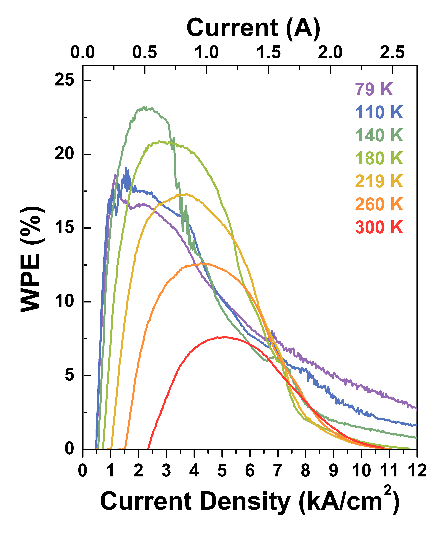
\includegraphics[width=2.75in]{2well-WPE_tifeps}%
\label{2well:WPE}}%
\caption[Performance data for the two injector well structure]{\tn{\textbf{Performance data for the three injector well structure.}} \tn{(a)} Representative normalized spectra of the two injector well structure for $T_{sink}=79~\tn{K}$ and \tn{300~K} near threshold.  Characteristic temperature $T_0$ \tn{(b)} and pulsed wall-plug efficiency \tn{(c)} for the two injector well $7.5~\tn{\um}\times3~\tn{mm}$ BH laser device that corresponds to the Fig.~\ref{2well:laser_a529ZB} LIV data.}%
\label{2well:performance}%
\end{figure}

Even with all of the unique features of the present device, performance is comparable to the field's best designs.  For the BH laser device described by the Figs.~\ref{2well:laser_a529ZB} and \ref{2well:performance} data, pulsed total output power peaks at 3.9~W at 180~K, while room temperature output power is 1.4~W.  Low temperature output power in these devices is severely limited by the pulse instabilities previously discussed.  Threshold current density is 460~A/cm$^2$ at 80~K, and reaches 2.3~kA/cm$^2$ at room temperature.  Figure~\ref{2well:T0} shows threshold behavior similar to the three injector well design.  As in the three injector well device, the $T_0$ approaching room temperature is relatively low at 113~K; the low temperature $T_0$~=~305~K.  Wall-plug efficiency---as shown in Fig.~\ref{2well:WPE}---peaks at 23.0\% for $T_{sink}$~=~140~K and 7.6\% at 300~K.  Again, wall-plug efficiency at low temperatures is limited by pulse instabilities.



\section{Conclusions and Future Directions}

\subsection{Summary}
In this chapter, I have presented our study on short injector region QC lasers, taking the approach of shrinking the conventional (approximately) seven well injector region to only two or three wells.  Making the active core gain region ``more dense'' with optical transitions by shortening the QC period length in principle leads to improvement in performance metrics associated with output power and efficiency. That performance should be improved for shorter QC period lengths should come as no surprise.  And recognizing the cascading effect of QC lasers, the field has a history of maximizing (and optimizing) the number of stacked QC periods \cite{Gmachl:JSTQE:1999}.

Through this study of short injectors, we have observed a host of unique effects in QC lasers.  Pronounced NDR is observed, where the presence of stimulated emission impacts the operating configuration of the laser band structure.  Turn-off mechanisms---increases in differential resistance---are observed at constant voltages with temperature, in addition to the more conventional turn-off features observed at constant current.  These effects can be attributed to two distinctive characteristics of the short injector designs presented here: enhanced ``coupling'' of neighboring active regions due to the close proximity afforded by the extremely abbreviated injector regions; and the highly discreet nature of the injector region energy states. %that we attribute to an enhanced coupling of active regions and the highly discrete nature of the energy states involved in transport throughout the structure.  We have seen NDR.  The NDR is from the coupling.  It turns on before it should.  We have seen other evidence of active region--active region coupling, like the constant voltage effect.

The observation of these new phenomena provide additional insight into the mechanisms of QC laser operation.  These effects are particularly relevant when designing QC lasers having minimalized injector regions.  Much of what we have observed confirms that such abbreviated QC structures behave in many ways similar to the classical superlattice.  For example, the highly discrete nature of individual states becomes particularly relevant, as well as the need to damp pulse instabilities \cite{Savvidis:PRL:2004} associated with shifting charge distributions.  The pronounced NDR of the three injector well laser and its successful operation at a lowered field demonstrates the effect of stimulated emission on electron distributions and energy state lifetimes.  It brings into question the field's perception that electrons always pool in the lowest energy state, and that states must be aligned in a downward order before sufficient transport occurs for laser action.

%that lasers can operate with lower states in the injector region, and that electrons don't necessarily pool like what might be expected when lasing dynamics (the effect of stimulated emission on electron distributions and state lifetimes) are involved; that is, a state with a dynamic lifetime can actively change the band structure configuration.

%Additional insight into QC structures and lasing.
%Evidence of direct, rapid, ballistic transport across injector regions.  Shrinking injector regions to the size of the electron.  Highly discrete states, so each one counts.

Even with these effects, we have shown data comparable with state-of-the-art designs.  We expect future improvement for designs making cognizant use of these discoveries.

\subsection{Future Direction: Higher performance QC lasers}

Notwithstanding the many of unique features discussed in this chapter---some of which may have limited performance in these first-generation short injector devices---optimizing length and other structural elements in injector regions holds great potential for improving QC wall-plug efficiency and overall performance.  As of this writing, we have achieved 46.6\% wall-plug efficiency from a $\lambda_0=4.6$ \um\ QC laser that incorporates a short injector ($L_p=346$~\AA) with further improvement of injector region structure \cite{Khurgin:APL:2009}.  While this record efficiency is for $T_{sink}=80$~K, the result is a discontinuity in the incremental performance improvements of the last several years.  Performance is rapidly improving, and shortened injectors are playing a key role.


\subsection{Future Direction: Improving temperature performance}

The two short injector designs herein presented, along with other short injector structures not yet reported, have shown consistently low characteristic temperatures: $T_0\leq120$~K.  Ultimately, such low $T_0$ will prove untenable for the commercially practicable case of room temperature high performance lasers.  The systematic nature of these low $T_0$s may ultimately a clue to the origin of the problem.  While we commonly refer to threshold current densities $J_{th}$, we rarely consider threshold voltage $V_{th}$.  Systematic examinations of $V_{th}$ reveal that this value is remarkably constant with temperature.  This isn't surprising: in a QCL, a sufficient voltage must be applied to achieve the desired---designed---band alignment.  As the temperature increases in a laser core, the thermal distribution of electrons increases and the energy levels broaden.  This commonly results in the ``softening'' of the initial IV turn-on with temperature.  The slower the turn-on, the more current must be pumped through the laser to reach $V_{th}$.

It is possible that short injector regions are making this effect worse.  Where a conventional, long injector region provides a sizeable barrier over which thermal electrons must ``jump'' before they can contribute to such a ``thermal current,'' a short injector imparts an ostensibly smaller barrier.  That is, as the injector region is shortened, energy states in adjacent active regions more readily mix, increasing the tunneling probability--and therefore thermal transport rate--between.  Thus, the very same mechanisms that at low temperature make short injectors so compelling create an additional hurdle at higher temperatures.

With an understanding of the source of the problem, solutions can be devised.  Ideally, what is needed is a way to block electron transport until $V_{th}$ is reached.  Indeed, we may have demonstrated just such a mechanism in this chapter.  We showed that transit times are sufficiently fast for short injector structures that a significant amount of injected current is supported without the aid of doped carriers.  Specifically, the three well injector structure exhibited current transport at a field where the free electrons contributed from doping were still trapped in the active region ground state.  Capitalizing on this effect could be the key to realizing the promise of short injector structures.



%\bibliographystyle{kale3}
%\bibliography{biblio}
%\end{document} 